\section{Background}

While discussing the `digital fitness' of languages \cite{soria2016fostering}
% TG % with respect to their usage, dissemination and accessibility on the web, resp., of web resources for speakers of that languages, emphasis is often put on parameters such as the size of the speaker community and the number (or existence) of resources and tools. We consider this perspective, however, to be a little bit too narrow, in that the existence of, say, spell checkers, chatbots, MT technology, dictionaries or just plain texts may not be equally helpful to all speakers of the language under consideration, depending on the \emph{degree of internal diversity} of the language, the orthographies used to write its dialects, and the degree of standardization accepted by the speaker community. 
with respect to their usage, dissemination and accessibility of web resources for speakers of that languages, emphasis is often put on speaker community size and the number (or existence) of resources and tools. However, such measures can be too narrow since tools like spell checkers, chatbots, MT technology, dictionaries, or plain texts may not be equally  helpful to all speakers due to the language's \emph{degree of internal diversity}, varying orthographies, and accepted standards.
% TG % As a point in case, we describe an approach for creating both a machine-readable dictionary and interdialectal links for Low German (Low Saxon, ISO 639-2 \code{nds}), a European minority language with a high degree of phonological, morphological and orthographic diversity. It is to be noted that, although Modern Low German has developed a vibrant production of (regional) literature since about 1800, it not only lacks a written standard, but also corpora, machine-readable dictionaries, and interdialectal dictionaries. More importantly, it also has a deficit of parallel texts, and in particular, texts attested in more than one variety of Low German, so that most modern NLP technology tailored towards exploiting parallel text are not applicable. Likewise, there is a problem in applying off-the-shelf embeddings or LLMs due to the lack of consistent training data on the web.
As a point in case, we describe an approach for creating both a machine-readable dictionary and interdialectal links for Low German (Low Saxon, ISO 639-2 \code{nds}), a European minority language with considerable phonological, morphological and orthographic diversity. Although Modern Low German has developed vibrant (regional) literature since about 1800, it lacks a written standard, corpora, machine-readable and interdialectal dictionaries, and, in particular, parallel texts and texts attested in more than one variety of Low German, limiting modern NLP applications. Likewise, off-the-shelf embeddings or LLMs are impractical due to inconsistent web training data.\footnote{
    We are aware of only one larger-scale experiment on using LLMs for Low German. According to public reports, however, this largely failed to achieve its preliminary goals after a 6 month piloting period, and was abandoned in August 2024, cf. \url{https://www.ndr.de/kultur/norddeutsche_sprache/niederdeutsch/Pepper-Blog-34-Neue-wissenschaftliche-Wege,pepperblog180.html}.
}

% TG % Without artifically enforcing normalization and standardization, what is needed to develop effective NLP support for Low German is a digital Rosetta stone that allows us to leverage materials from different language varieties and to access them in a uniform way. This can by done by means of language normalization, but this has been a controversial topic in the past \cite{Christiansen1975}, and -- beyond the level of geographically confined regions -- seems to be largely rejected by the speaker community. Instead, we focus on technologies to create `non-invasive' synergies between dialect-specific resources on the web, by creating links between regional dictionaries, and by providing a mapping routine capable to \emph{spot} formally corresponding words in different dialects which can subsequently be linked. In this paper, we primarily focus on the first aspect, on providing adequate methods of access to such data for both humans and machines. On the one hand, web-scale linking across physically dispersed data sources can be naturally addressed by means of RDF and Linked Open Data technology \cite[p.3-9]{cimiano2020linguistic}, but providing our data as Linguistic Linked Open Data (LLOD) involves a number of technological challenges in data modelling (of the dictionaries and inter-dictionary links), in accessibility (i.e., readability for a human), and also in terms of legal constraints (in fact, most dictionaries freely accessible over the web adopt a proprietary licensing model so that their content cannot be directly used -- but it can be linked).
Without enforcing normalization and standardization, effective NLP support for Low German requires a “digital Rosetta stone” that allows us to integrate diverse language varieties uniformly. Although language normalization is possible, it has been a controversial topic \cite{Christiansen1975}, and -- beyond the level of geographically confined regions -- seems to be largely rejected by the speaker community. Instead, we focus on creating `non-invasive' synergies between dialect-specific resources by linking regional dictionaries and providing a mapping routine capable of \emph{spotting} formally corresponding words across dialects. In this paper, we primarily focus on methods to access such data for both humans and machines. While web-scale linking of dispersed data sources can be addressed using RDF and Linked Open Data technology \cite[p.3-9]{cimiano2020linguistic}, providing our data as Linguistic Linked Open Data (LLOD) involves a number of challenges in data modeling (of the dictionaries and inter-dictionary links), accessibility (i.e., readability for a human), and legal constraints (since many online dictionaries use proprietary licenses that restrict direct use, but linking is permitted).

% TG % Low German or Low Saxon (self-designation \word{Plattdüütsch}, \word{Nedersassisch} or \word{Nedersaksisch}) is a West Germanic language historically spoken in northern Germany, the Netherlands and the southern coast of the Baltic Sea. It is closely related to and has been in continuous contact with Dutch, High German and Frisian, but followed its own developmental trajectory since its first recorded texts from the 9th c. CE \cite{price-2010-heliand-phd}). It is recognized as a regional language and protected under the European Charter for Regional or Minority Languages (ECRML). 
Low German or Low Saxon (self-designation \word{Plattdüütsch}, \word{Nedersassisch} or \word{Nedersaksisch}) is a West Germanic language historically spoken in northern Germany, the Netherlands and the southern coast of the Baltic Sea. Closely related to Dutch, High German and Frisian, it has followed its own developmental trajectory since its first recorded texts from the 9th c. CE \cite{price-2010-heliand-phd} and is protected under the European Charter for Regional or Minority Languages (ECRML).
% TG % Historically, (Middle) Low German served as a lingua franca around the Baltic Sea. However, with High German (in Germany) and Dutch (in the Netherlands) replacing it since the 17th c. as the dominant languages of education, administration, and media, it is now considered threatened (vulnerable) \cite[p.25]{moseley2010atlas}. While it still has millions of passive speakers, active speakers are far fewer and to a large extent senior citizens \cite{AdlerEhlersGoltzetal.2019}, so that one of the most pressing issues facing Low German today is transmission to the next generation of speakers. This requires didactic and educational material, but digital tools. Yet, even basic NLP tools like spell checkers, machine translation, speech recognition, and text-to-speech systems are effectively absent. A major challenge here is the fragmentation of the modern dialects of Low German, which diverged greatly since the Middle Ages (Tab. \ref{tab-dialects-and-isocodes}). Some, mostly northern, dialects lost the unvoiced vowels of Middle Low German (and thus parts of their morphological inventory), while others retained them (along with the four nominal cases, the present subjunctive, etc.). Alongside this north-south division, there also exists an west-east division that reflects the expansion of Low German towards formerly Slavic territories during the Middle Ages, with modern Western dialects using a uniform verbal plural in \word{-(e)t}, and Eastern dialects using a verbal plural in \word{-en}. The dialects east of the river Oder ceased to be spoken after WWII, but gave rise to emmigrant varieties such as Pomerano (a regionally recognized minority language in Brazil) and Plautdietsch (spoken by the Mennonite diaspora in the Americas).
Historically, (Middle) Low German served as a lingua franca around the Baltic Sea. However, with High German (in Germany) and Dutch (in the Netherlands) replacing it as the dominant languages of education, administration, and media since the 17th c., it is now considered threatened (vulnerable) \cite[p.25]{moseley2010atlas}. While it still has millions of passive speakers, active speakers are far fewer and to a large extent elderly citizens \cite{AdlerEhlersGoltzetal.2019}, making intergenerational transmission a key challenge. This demands both educational material and digital tools, yet basic NLP tools such as spell checkers, machine translation, speech recognition, and text-to-speech systems are effectively absent. The fragmentation of modern Low German dialects -- which have diverged greatly since the Middle Ages (Tab. \ref{tab-dialects-and-isocodes}) -- further complicates digital communication. For example, some northern dialects lost the unvoiced vowels of Middle Low German (and thus parts of their morphological inventory), while others preserved them. Alongside this north-south division, there also exists an west-east division that reflects the expansion of Low German towards formerly Slavic territories during the Middle Ages, with Western dialects (historically) using a uniform verbal plural in \word{-(e)t}, and Eastern dialects (historically) using a verbal plural in \word{-en}. Dialects east of the Oder ceased after WWII but gave rise to emigrant varieties like Pomerano (a regionally recognized minority language in Brazil) and Plautdietsch (spoken by the Mennonite diaspora, predominantly in the Americas).

\begin{table}
    \centering
    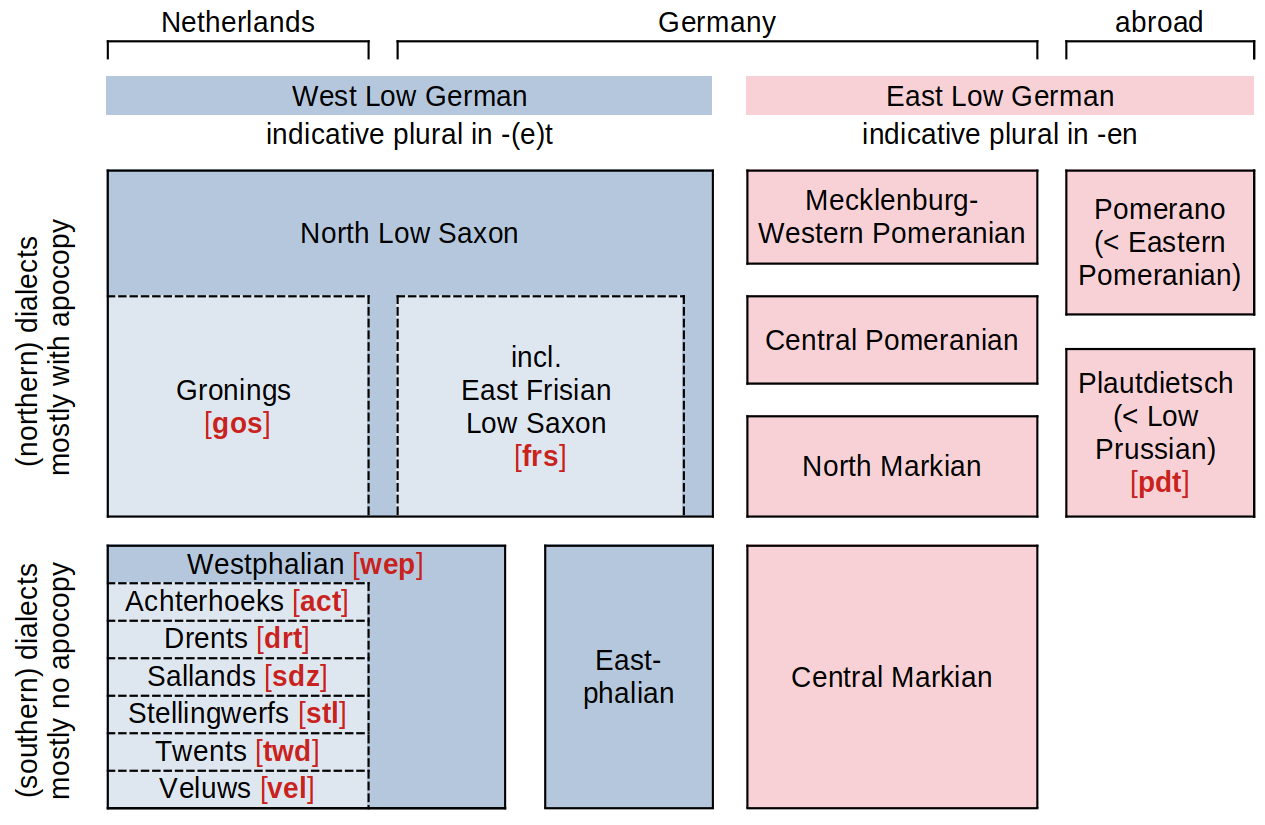
\includegraphics[width=1.0\linewidth]{img/dialects-and-iso632-codes.png}
    \caption{Major dialects of Low German (ISO 639-2 \code{nds}), with regional ISO 639-3 codes in red square brackets.}
    \label{tab-dialects-and-isocodes}
\end{table}

% TG % This particularization makes it difficult to use the language in digital communication, reducing its visibility and usability in the modern world -- or to develop tools and resources to facilitate such applications or to support its speakers and learners. The absence of NLP tools also hinders academic research, automated language processing, and efforts to create digital content in Low German. Despite these challenges, Low German enjoys cultural and regional recognition. Efforts to revitalize the language include educational programs, literature, radio broadcasts, and online initiatives. However, without stronger support on many levels, the survival of Low German as a living language remains uncertain. In fact, social networks and digital language resources may play a role in transmission and revitalization of the Low German language, and indeed, this is what we see for other minority languages all over the world. To preserve Low German, more work is needed to integrate it into digital spaces. Developing NLP tools, expanding online resources, and increasing its presence in modern media are crucial steps in ensuring that Low German remains a functional and thriving language for future generations. At the moment, however, even the most basic NLP resources are still lacking, with a deficit in corpora \cite{siewert2021towards}, the complete lack of parallel corpora, and no machine-readable dictionaries. 

This fragmentation makes it difficult to use the language in digital communication -- reducing its visibility and usability in the modern world -- and to develop tools for its Low German speakers and learners. The absence of NLP tools also hinders academic research, automated language processing, and digital content creation. Despite these challenges, Low German enjoys cultural and regional recognition. Efforts to revitalize the language include educational programs, literature, radio broadcasts, and online initiatives. These resources may play a role in transmission and revitalization of the Low German language, and indeed, this is what we see for other minority languages all over the world. However, to preserve Low German, more work is needed to integrate it into digital spaces. Developing NLP tools, expanding online resources, and boosting media presence are crucial for its survival as a living language. Currently, fundamental NLP resources are lacking, including corpora \cite{siewert2021towards}, parallel corpora, and machine-readable dictionaries. 

% TG % A \emph{machine-readable dictionary (MRD)} is a structured lexical resource designed for computational use rather than human readability. Unlike traditional dictionaries, MRDs are formatted in a way that allows software applications to process and analyze linguistic data efficiently. They store information such as word meanings, grammatical properties, pronunciations, and translations in a structured manner to facilitate the development of downstream applications. For low-resource languages, \emph{machine-readable dictionaries} (MRDs) play a crucial role in developing foundational NLP technologies. In particular, this is the case for language varieties that have been the subject of linguistic research in the past (so that word lists or dictionaries are available), but that have been largely neglected by NLP or corpus linguistics (so that no digital corpus data is available).
A \emph{machine-readable dictionary (MRD)} is a lexical resource structured for computational use rather than human readability. Unlike traditional dictionaries, MRDs are formatted in a way that allows software applications to process and analyze linguistic data efficiently. They store information such as word meanings, grammatical properties, pronunciations, and translations in a structured manner to facilitate the development of downstream applications. For low-resource languages, MRDs play a crucial role in developing foundational NLP technologies. In particular, this is the case for language varieties that have been the subject of linguistic research in the past (so that word lists or dictionaries are available), but that have been largely neglected by NLP or corpus linguistics (so that no digital corpus data is available). 
% TG % As for existing MRDs, we are not aware of any Low German data except for isolated Low German terms in foreign-language editions of DBnary \cite{serasset2014dbnary}, however, this crowd-sourced, it does not adhere to a consistent orthography and is thus not considered here.
We are unaware of any existing comprehensive Low German MRD, aside from isolated Low German terms in foreign-language editions of DBnary \cite{serasset2014dbnary} (which is crowd-sourced and inconsistent). 
% TG % This paper describes the development of a prototypical interdialectal MRD for Low German, consisting of two parts, a core created from a dictionary of the North Low Saxon dialekt of Dithmarschen \cite[further WöWö]{neuber-2001-woerner-woer}, republished 2019 as \word{Frie' Woor} `freeware' as digital-born DOCX and PDF files. To the best of our knowledge, this is the only digital dictionary of a regional variety of Low German in Germany for which free redistribution is explicitly allowed. \footnote{There also is a multi-dialectal Low German Wiktionary under CC BY-NC-SA. However, this is crowd-sourced and orthographically inconsistent and thus not considered here.}
This paper describes the development of a prototypical interdialectal MRD for Low German, consisting of two parts, a core built from a North Low Saxon dictionary of Dithmarschen \cite[further WöWö]{neuber-2001-woerner-woer}, republished in 2019 as \word{Frie' Woor} `freeware' digital-born DOCX and PDF files. To the best of our knowledge, this is the only digital dictionary of a regional variety of Low German in Germany for which free redistribution is explicitly allowed.\footnote{
    There also is a multi-dialectal Low German Wiktionary under CC BY-NC-SA. However, this is crowd-sourced, and thus orthographically inconsistent and not considered here. 
}
% TG % This is then complemented by interdialectal links. For these, we can build on a number of digital dictionaries in existence, but each pertains to a different variety and all are designed for human consumption, and not for subsequent use in natural language processing. In addition to that, most of these are copyright-protected, either explicitly or by default copyright (if copyright is undeclared). The approach we suggest can, however, be extended to other Low German dictionaries and dialects if copyright can be secured.
This is complemented by interdialectal links, derived from various digital dictionaries, though all are designed for human consumption, and not for subsequent use in natural language processing. In addition, most of these are copyright-protected, either explicitly or by default copyright (if copyright is undeclared). Our approach can, however, be extended to other Low German dictionaries and dialects if copyright can be secured.
    
A key technology for building structured and interoperable MRDs is \emph{OntoLex-Lemon}, an RDF vocabulary  designed for representing lexical and semantic data on the web \cite{mccrae2017ontolex}. OntoLex allows lexicons to be linked to external knowledge bases and other linguistic resources, enhancing interoperability. It uses the Resource Description Framework \cite[RDF]{beckett2014rdf}, a W3C standard to provide a flexible, graph-based data model that enables rich semantic annotations and structured linguistic relationships. Together, these technologies ensure that dictionaries for low-resource languages are not isolated but can be \emph{integrated into broader linguistic ecosystems}, facilitating cross-linguistic research and NLP. By leveraging OntoLex and RDF, MRDs for low-resource languages can be built in a way that supports automated processing, encourages digital preservation, and enables their incorporation into modern NLP applications. 
These technologies make it easier to link lexical resources across languages, ensuring that low-resource languages gain better representation in computational linguistics and digital tools. As such, OntoLex has been a cornerstone for integrating lexical data into the Linguistic Linked Open Data cloud \cite{declerck2018towards}. 

The \emph{Linguistic Linked Open Data (LLOD)} cloud \cite{chiarcos2011towards,pareja2019development,cimiano2020linguistic} is an interlinked network of linguistic resources following Linked Data principles \cite{bizer2009linked}.\footnote{
    The native home of the LLOD cloud diagram is \url{https://linguistic-lod.org/}. Since 2018, it has been formally integrated into the LOD cloud diagram and is currently provided as a separate LOD subcloud under \url{https://lod-cloud.net/\#linguistic}.
} 
It provides a semantic web-based infrastructure for representing and integrating linguistic data, including lexicons, corpora, terminologies, and ontologies.
A key advantage of the LLOD approach is its ability to connect diverse linguistic datasets, making them accessible for computational use. 
%Resources such as OntoLex-Lemon facilitate the representation of lexicons, while linguistic ontologies like OLiA (Ontologies of Linguistic Annotations) provide standardized annotation frameworks \cite{chiarcos2012olia}. 
The LLOD cloud benefits low-resource languages by linking their limited linguistic data to richer datasets, fostering NLP development and linguistic research. By structuring linguistic resources using open standards, the LLOD cloud contributes to the creation of multilingual and interoperable NLP systems, supporting tasks such as machine translation, semantic search, and corpus analysis. For languages with scarce and scattered data, LLOD is vital for digital preservation and computational access to linguistic knowledge. 

%, also cf. ACoLi dictionary graphs. However, PanDoc data is generally of mixed quality, as it is largely based on automated OCR. Wiktionary data is crowdsourced, and for a language without a written standard, this data is too unsystematic to be used and reliably linked with other lexical resources, as it freely mixes mixes regional and author-specific orthographies.
%In addition to these dictionaries, there are many print dictionaries, also in the public domain, but not reliably digitized. 

